\documentclass[a4paper,11pt]{report}

%%%%%%%%%%%%%%%%%%%%%%%%%%%%%%%%%
% PACKAGE IMPORTS
%%%%%%%%%%%%%%%%%%%%%%%%%%%%%%%%%
\usepackage[tmargin=2cm,rmargin=1in,lmargin=1in,margin=0.85in,bmargin=2cm,footskip=.2in]{geometry}
\usepackage[none]{hyphenat}
\usepackage{amsmath,amsfonts,amsthm,amssymb,mathtools}
\allowdisplaybreaks
\usepackage{undertilde}
\usepackage{xfrac}
\usepackage[makeroom]{cancel}
\usepackage{mathtools}
\usepackage{bookmark}
\usepackage{enumitem}
\usepackage{kbordermatrix}
\renewcommand{\kbldelim}{(} % Change left delimiter to (
\renewcommand{\kbrdelim}{)} % Change right delimiter to )
\usepackage{hyperref,theoremref}
\hypersetup{
	pdftitle={Assignment},
	colorlinks=true, linkcolor=doc!90,
	bookmarksnumbered=true,
	bookmarksopen=true
}
\usepackage[most,many,breakable]{tcolorbox}
\usepackage{xcolor}
\usepackage{varwidth}
\usepackage{varwidth}
\usepackage{etoolbox}
%\usepackage{authblk}
\usepackage{nameref}
\usepackage{multicol,array}
\usepackage{tikz-cd}
\usepackage[ruled,vlined,linesnumbered]{algorithm2e}
\usepackage{comment} % enables the use of multi-line comments (\ifx \fi) 
\usepackage{import}
\usepackage{xifthen}
\usepackage{pdfpages}
\usepackage{svg}
\usepackage{transparent}
\usepackage{pgfplots}
\pgfplotsset{compat=1.18}
\usetikzlibrary{calc}
\usetikzlibrary{graphs}
\usetikzlibrary{graphs.standard}
% \usetikzlibrary{graphdrawing}

\newcommand\mycommfont[1]{\footnotesize\ttfamily\textcolor{blue}{#1}}
\SetCommentSty{mycommfont}
\newcommand{\incfig}[1]{%
    \def\svgwidth{\columnwidth}
    \import{./figures/}{#1.pdf_tex}
}


\usepackage{tikzsymbols}
% \renewcommand\qedsymbol{$\Laughey$}

\definecolor{commentgreen}{RGB}{2,112,10}
%%
%% Julia definition (c) 2014 Jubobs
%%
\lstdefinelanguage{Julia}%
  {morekeywords={abstract,break,case,catch,const,continue,do,else,elseif,%
      end,export,false,for,function,immutable,import,importall,if,in,%
      macro,module,otherwise,quote,return,switch,true,try,type,typealias,%
      using,while},%
   sensitive=true,%
   alsoother={$},%
   morecomment=[l]\#,%
   morecomment=[n]{\#=}{=\#},%
   morestring=[s]{"}{"},%
   morestring=[m]{'}{'},%
}[keywords,comments,strings]%

\lstset{%
    language        	= Julia,
    basicstyle      	= \ttfamily,
    keywordstyle    	= \bfseries\color{blue},
    stringstyle     	= \color{magenta},
    commentstyle    	= \color{commentgreen},
    showstringspaces	= false,
		numbers						= left,
		tabsize						= 4,
}

\definecolor{stringyellow}{RGB}{227, 78, 48}
%% 
%% Shamelessly stolen from Vivi on Stackoverflow
%% https://tex.stackexchange.com/questions/75116/what-can-i-use-to-typeset-matlab-code-in-my-document
%%
\lstset{language=Matlab,%
    %basicstyle=\color{red},
    breaklines=true,%
    morekeywords={matlab2tikz},
		morekeywords={subtitle}
    keywordstyle=\color{blue},%
    morekeywords=[2]{1}, keywordstyle=[2]{\color{black}},
    identifierstyle=\color{black},%
    stringstyle=\color{stringyellow},
    commentstyle=\color{commentgreen},%
    showstringspaces=false,%without this there will be a symbol in the places where there is a space
    numbers=left,%
		firstnumber=1,
    % numberstyle={\tiny \color{black}},% size of the numbers
    % numbersep=9pt, % this defines how far the numbers are from the text
    emph=[1]{for,end,break},emphstyle=[1]\color{red}, %some words to emphasise
    %emph=[2]{word1,word2}, emphstyle=[2]{style},    
}

%% 
%% Shamelessly stolen from egreg on Stackoverflow
%% https://tex.stackexchange.com/questions/280681/how-to-have-multiple-lines-of-intertext-within-align-environment
%%
\newlength{\normalparindent}
\AtBeginDocument{\setlength{\normalparindent}{\parindent}}
\newcommand{\longintertext}[1]{%
  \intertext{%
    \parbox{\linewidth}{%
      \setlength{\parindent}{\normalparindent}
      \noindent#1%
    }%
  }%
}

%\usepackage{import}
%\usepackage{xifthen}
%\usepackage{pdfpages}
%\usepackage{transparent}

%%%%%%%%%%%%%%%%%%%%%%%%%%%%%%
% SELF MADE COLORS
%%%%%%%%%%%%%%%%%%%%%%%%%%%%%%
\definecolor{myg}{RGB}{56, 140, 70}
\definecolor{myb}{RGB}{45, 111, 177}
\definecolor{myr}{RGB}{199, 68, 64}
\definecolor{mytheorembg}{HTML}{F2F2F9}
\definecolor{mytheoremfr}{HTML}{00007B}
\definecolor{mylenmabg}{HTML}{FFFAF8}
\definecolor{mylenmafr}{HTML}{983b0f}
\definecolor{mypropbg}{HTML}{f2fbfc}
\definecolor{mypropfr}{HTML}{191971}
\definecolor{myexamplebg}{HTML}{F2FBF8}
\definecolor{myexamplefr}{HTML}{88D6D1}
\definecolor{myexampleti}{HTML}{2A7F7F}
\definecolor{mydefinitbg}{HTML}{E5E5FF}
\definecolor{mydefinitfr}{HTML}{3F3FA3}
\definecolor{notesgreen}{RGB}{0,162,0}
\definecolor{myp}{RGB}{197, 92, 212}
\definecolor{mygr}{HTML}{2C3338}
\definecolor{myred}{RGB}{127,0,0}
\definecolor{myyellow}{RGB}{169,121,69}
\definecolor{myexercisebg}{HTML}{F2FBF8}
\definecolor{myexercisefg}{HTML}{88D6D1}

%%%%%%%%%%%%%%%%%%%%%%%%%%%%
% TCOLORBOX SETUPS
%%%%%%%%%%%%%%%%%%%%%%%%%%%%
\setlength{\parindent}{0pt}

%================================
% THEOREM BOX
%================================
\tcbuselibrary{theorems,skins,hooks}
\newtcbtheorem[number within=section]{Theorem}{Theorem}
{%
	enhanced,
	breakable,
	colback = mytheorembg,
	frame hidden,
	boxrule = 0sp,
	borderline west = {2pt}{0pt}{mytheoremfr},
	sharp corners,
	detach title,
	before upper = \tcbtitle\par\smallskip,
	coltitle = mytheoremfr,
	fonttitle = \bfseries\sffamily,
	description font = \mdseries,
	separator sign none,
	segmentation style={solid, mytheoremfr},
}
{th}

\tcbuselibrary{theorems,skins,hooks}
\newtcbtheorem[number within=chapter]{theorem}{Theorem}
{%
	enhanced,
	breakable,
	colback = mytheorembg,
	frame hidden,
	boxrule = 0sp,
	borderline west = {2pt}{0pt}{mytheoremfr},
	sharp corners,
	detach title,
	before upper = \tcbtitle\par\smallskip,
	coltitle = mytheoremfr,
	fonttitle = \bfseries\sffamily,
	description font = \mdseries,
	separator sign none,
	segmentation style={solid, mytheoremfr},
}
{th}


\tcbuselibrary{theorems,skins,hooks}
\newtcolorbox{Theoremcon}
{%
	enhanced
	,breakable
	,colback = mytheorembg
	,frame hidden
	,boxrule = 0sp
	,borderline west = {2pt}{0pt}{mytheoremfr}
	,sharp corners
	,description font = \mdseries
	,separator sign none
}

%================================
% Corollery
%================================
\tcbuselibrary{theorems,skins,hooks}
\newtcbtheorem[number within=section]{Corollary}{Corollary}
{%
	enhanced
	,breakable
	,colback = myp!10
	,frame hidden
	,boxrule = 0sp
	,borderline west = {2pt}{0pt}{myp!85!black}
	,sharp corners
	,detach title
	,before upper = \tcbtitle\par\smallskip
	,coltitle = myp!85!black
	,fonttitle = \bfseries\sffamily
	,description font = \mdseries
	,separator sign none
	,segmentation style={solid, myp!85!black}
}
{th}
\tcbuselibrary{theorems,skins,hooks}
\newtcbtheorem[number within=chapter]{corollary}{Corollary}
{%
	enhanced
	,breakable
	,colback = myp!10
	,frame hidden
	,boxrule = 0sp
	,borderline west = {2pt}{0pt}{myp!85!black}
	,sharp corners
	,detach title
	,before upper = \tcbtitle\par\smallskip
	,coltitle = myp!85!black
	,fonttitle = \bfseries\sffamily
	,description font = \mdseries
	,separator sign none
	,segmentation style={solid, myp!85!black}
}
{th}

%================================
% LENMA
%================================
\tcbuselibrary{theorems,skins,hooks}
\newtcbtheorem[number within=section]{Lenma}{Lenma}
{%
	enhanced,
	breakable,
	colback = mylenmabg,
	frame hidden,
	boxrule = 0sp,
	borderline west = {2pt}{0pt}{mylenmafr},
	sharp corners,
	detach title,
	before upper = \tcbtitle\par\smallskip,
	coltitle = mylenmafr,
	fonttitle = \bfseries\sffamily,
	description font = \mdseries,
	separator sign none,
	segmentation style={solid, mylenmafr},
}
{th}

\tcbuselibrary{theorems,skins,hooks}
\newtcbtheorem[number within=chapter]{lenma}{Lenma}
{%
	enhanced,
	breakable,
	colback = mylenmabg,
	frame hidden,
	boxrule = 0sp,
	borderline west = {2pt}{0pt}{mylenmafr},
	sharp corners,
	detach title,
	before upper = \tcbtitle\par\smallskip,
	coltitle = mylenmafr,
	fonttitle = \bfseries\sffamily,
	description font = \mdseries,
	separator sign none,
	segmentation style={solid, mylenmafr},
}
{th}

%================================
% PROPOSITION
%================================
\tcbuselibrary{theorems,skins,hooks}
\newtcbtheorem[number within=section]{Prop}{Proposition}
{%
	enhanced,
	breakable,
	colback = mypropbg,
	frame hidden,
	boxrule = 0sp,
	borderline west = {2pt}{0pt}{mypropfr},
	sharp corners,
	detach title,
	before upper = \tcbtitle\par\smallskip,
	coltitle = mypropfr,
	fonttitle = \bfseries\sffamily,
	description font = \mdseries,
	separator sign none,
	segmentation style={solid, mypropfr},
}
{th}

\tcbuselibrary{theorems,skins,hooks}
\newtcbtheorem[number within=chapter]{prop}{Proposition}
{%
	enhanced,
	breakable,
	colback = mypropbg,
	frame hidden,
	boxrule = 0sp,
	borderline west = {2pt}{0pt}{mypropfr},
	sharp corners,
	detach title,
	before upper = \tcbtitle\par\smallskip,
	coltitle = mypropfr,
	fonttitle = \bfseries\sffamily,
	description font = \mdseries,
	separator sign none,
	segmentation style={solid, mypropfr},
}
{th}

%================================
% CLAIM
%================================
\tcbuselibrary{theorems,skins,hooks}
\newtcbtheorem[number within=section]{claim}{Claim}
{%
	enhanced
	,breakable
	,colback = myg!10
	,frame hidden
	,boxrule = 0sp
	,borderline west = {2pt}{0pt}{myg}
	,sharp corners
	,detach title
	,before upper = \tcbtitle\par\smallskip
	,coltitle = myg!85!black
	,fonttitle = \bfseries\sffamily
	,description font = \mdseries
	,separator sign none
	,segmentation style={solid, myg!85!black}
}
{th}

%================================
% Exercise
%================================
\tcbuselibrary{theorems,skins,hooks}
\newtcbtheorem[number within=section]{Exercise}{Exercise}
{%
	enhanced,
	breakable,
	colback = myexercisebg,
	frame hidden,
	boxrule = 0sp,
	borderline west = {2pt}{0pt}{myexercisefg},
	sharp corners,
	detach title,
	before upper = \tcbtitle\par\smallskip,
	coltitle = myexercisefg,
	fonttitle = \bfseries\sffamily,
	description font = \mdseries,
	separator sign none,
	segmentation style={solid, myexercisefg},
}
{th}

\tcbuselibrary{theorems,skins,hooks}
\newtcbtheorem[number within=chapter]{exercise}{Exercise}
{%
	enhanced,
	breakable,
	colback = myexercisebg,
	frame hidden,
	boxrule = 0sp,
	borderline west = {2pt}{0pt}{myexercisefg},
	sharp corners,
	detach title,
	before upper = \tcbtitle\par\smallskip,
	coltitle = myexercisefg,
	fonttitle = \bfseries\sffamily,
	description font = \mdseries,
	separator sign none,
	segmentation style={solid, myexercisefg},
}
{th}

%================================
% EXAMPLE BOX
%================================
\newtcbtheorem[number within=section]{Example}{Example}
{%
	colback = myexamplebg
	,breakable
	,colframe = myexamplefr
	,coltitle = myexampleti
	,boxrule = 1pt
	,sharp corners
	,detach title
	,before upper=\tcbtitle\par\smallskip
	,fonttitle = \bfseries
	,description font = \mdseries
	,separator sign none
	,description delimiters parenthesis
}
{ex}

\newtcbtheorem[number within=chapter]{example}{Example}
{%
	colback = myexamplebg
	,breakable
	,colframe = myexamplefr
	,coltitle = myexampleti
	,boxrule = 1pt
	,sharp corners
	,detach title
	,before upper=\tcbtitle\par\smallskip
	,fonttitle = \bfseries
	,description font = \mdseries
	,separator sign none
	,description delimiters parenthesis
}
{ex}

%================================
% DEFINITION BOX
%================================
\newtcbtheorem[number within=section]{Definition}{Definition}{enhanced,
	before skip=2mm,after skip=2mm, colback=red!5,colframe=red!80!black,boxrule=0.5mm,
	attach boxed title to top left={xshift=1cm,yshift*=1mm-\tcboxedtitleheight}, varwidth boxed title*=-3cm,
	boxed title style={frame code={
					\path[fill=tcbcolback]
					([yshift=-1mm,xshift=-1mm]frame.north west)
					arc[start angle=0,end angle=180,radius=1mm]
					([yshift=-1mm,xshift=1mm]frame.north east)
					arc[start angle=180,end angle=0,radius=1mm];
					\path[left color=tcbcolback!60!black,right color=tcbcolback!60!black,
						middle color=tcbcolback!80!black]
					([xshift=-2mm]frame.north west) -- ([xshift=2mm]frame.north east)
					[rounded corners=1mm]-- ([xshift=1mm,yshift=-1mm]frame.north east)
					-- (frame.south east) -- (frame.south west)
					-- ([xshift=-1mm,yshift=-1mm]frame.north west)
					[sharp corners]-- cycle;
				},interior engine=empty,
		},
	fonttitle=\bfseries,
	title={#2},#1}{def}
\newtcbtheorem[number within=chapter]{definition}{Definition}{enhanced,
	before skip=2mm,after skip=2mm, colback=red!5,colframe=red!80!black,boxrule=0.5mm,
	attach boxed title to top left={xshift=1cm,yshift*=1mm-\tcboxedtitleheight}, varwidth boxed title*=-3cm,
	boxed title style={frame code={
					\path[fill=tcbcolback]
					([yshift=-1mm,xshift=-1mm]frame.north west)
					arc[start angle=0,end angle=180,radius=1mm]
					([yshift=-1mm,xshift=1mm]frame.north east)
					arc[start angle=180,end angle=0,radius=1mm];
					\path[left color=tcbcolback!60!black,right color=tcbcolback!60!black,
						middle color=tcbcolback!80!black]
					([xshift=-2mm]frame.north west) -- ([xshift=2mm]frame.north east)
					[rounded corners=1mm]-- ([xshift=1mm,yshift=-1mm]frame.north east)
					-- (frame.south east) -- (frame.south west)
					-- ([xshift=-1mm,yshift=-1mm]frame.north west)
					[sharp corners]-- cycle;
				},interior engine=empty,
		},
	fonttitle=\bfseries,
	title={#2},#1}{def}

%================================
% Solution BOX
%================================
\makeatletter
\newtcbtheorem{question}{Question}{enhanced,
	breakable,
	colback=white,
	colframe=myb!80!black,
	attach boxed title to top left={yshift*=-\tcboxedtitleheight},
	fonttitle=\bfseries,
	title={#2},
	boxed title size=title,
	boxed title style={%
			sharp corners,
			rounded corners=northwest,
			colback=tcbcolframe,
			boxrule=0pt,
		},
	underlay boxed title={%
			\path[fill=tcbcolframe] (title.south west)--(title.south east)
			to[out=0, in=180] ([xshift=5mm]title.east)--
			(title.center-|frame.east)
			[rounded corners=\kvtcb@arc] |-
			(frame.north) -| cycle;
		},
	#1
}{def}
\makeatother

%================================
% SOLUTION BOX
%================================
\makeatletter
\newtcolorbox{solution}{enhanced,
	breakable,
	colback=white,
	colframe=myg!80!black,
	attach boxed title to top left={yshift*=-\tcboxedtitleheight},
	title=Solution,
	boxed title size=title,
	boxed title style={%
			sharp corners,
			rounded corners=northwest,
			colback=tcbcolframe,
			boxrule=0pt,
		},
	underlay boxed title={%
			\path[fill=tcbcolframe] (title.south west)--(title.south east)
			to[out=0, in=180] ([xshift=5mm]title.east)--
			(title.center-|frame.east)
			[rounded corners=\kvtcb@arc] |-
			(frame.north) -| cycle;
		},
}
\makeatother

%================================
% Question BOX
%================================
\makeatletter
\newtcbtheorem{qstion}{Question}{enhanced,
	breakable,
	colback=white,
	colframe=mygr,
	attach boxed title to top left={yshift*=-\tcboxedtitleheight},
	fonttitle=\bfseries,
	title={#2},
	boxed title size=title,
	boxed title style={%
			sharp corners,
			rounded corners=northwest,
			colback=tcbcolframe,
			boxrule=0pt,
		},
	underlay boxed title={%
			\path[fill=tcbcolframe] (title.south west)--(title.south east)
			to[out=0, in=180] ([xshift=5mm]title.east)--
			(title.center-|frame.east)
			[rounded corners=\kvtcb@arc] |-
			(frame.north) -| cycle;
		},
	#1
}{def}
\makeatother

\newtcbtheorem[number within=chapter]{wconc}{Wrong Concept}{
	breakable,
	enhanced,
	colback=white,
	colframe=myr,
	arc=0pt,
	outer arc=0pt,
	fonttitle=\bfseries\sffamily\large,
	colbacktitle=myr,
	attach boxed title to top left={},
	boxed title style={
			enhanced,
			skin=enhancedfirst jigsaw,
			arc=3pt,
			bottom=0pt,
			interior style={fill=myr}
		},
	#1
}{def}

%================================
% NOTE BOX
%================================
\usetikzlibrary{arrows,calc,shadows.blur}
\tcbuselibrary{skins}
\newtcolorbox{note}[1][]{%
	enhanced jigsaw,
	colback=gray!20!white,%
	colframe=gray!80!black,
	size=small,
	boxrule=1pt,
	title=\textbf{Note:-},
	halign title=flush center,
	coltitle=black,
	breakable,
	drop shadow=black!50!white,
	attach boxed title to top left={xshift=1cm,yshift=-\tcboxedtitleheight/2,yshifttext=-\tcboxedtitleheight/2},
	minipage boxed title=1.5cm,
	boxed title style={%
			colback=white,
			size=fbox,
			boxrule=1pt,
			boxsep=2pt,
			underlay={%
					\coordinate (dotA) at ($(interior.west) + (-0.5pt,0)$);
					\coordinate (dotB) at ($(interior.east) + (0.5pt,0)$);
					\begin{scope}
						\clip (interior.north west) rectangle ([xshift=3ex]interior.east);
						\filldraw [white, blur shadow={shadow opacity=60, shadow yshift=-.75ex}, rounded corners=2pt] (interior.north west) rectangle (interior.south east);
					\end{scope}
					\begin{scope}[gray!80!black]
						\fill (dotA) circle (2pt);
						\fill (dotB) circle (2pt);
					\end{scope}
				},
		},
	#1,
}

%%%%%%%%%%%%%%%%%%%%%%%%%%%%%%
% SELF MADE COMMANDS
%%%%%%%%%%%%%%%%%%%%%%%%%%%%%%
\newcommand{\thm}[2]{\begin{Theorem}{#1}{}#2\end{Theorem}}
\newcommand{\cor}[2]{\begin{Corollary}{#1}{}#2\end{Corollary}}
\newcommand{\mlenma}[2]{\begin{Lenma}{#1}{}#2\end{Lenma}}
\newcommand{\mprop}[2]{\begin{Prop}{#1}{}#2\end{Prop}}
\newcommand{\clm}[3]{\begin{claim}{#1}{#2}#3\end{claim}}
\newcommand{\wc}[2]{\begin{wconc}{#1}{}\setlength{\parindent}{1cm}#2\end{wconc}}
\newcommand{\thmcon}[1]{\begin{Theoremcon}{#1}\end{Theoremcon}}
\newcommand{\ex}[2]{\begin{Example}{#1}{}#2\end{Example}}
\newcommand{\dfn}[2]{\begin{Definition}[colbacktitle=red!75!black]{#1}{}#2\end{Definition}}
\newcommand{\dfnc}[2]{\begin{definition}[colbacktitle=red!75!black]{#1}{}#2\end{definition}}
\newcommand{\qs}[2]{\begin{question}{#1}{}#2\end{question}}
\newcommand{\pf}[2]{\begin{myproof}[#1]#2\end{myproof}}
\newcommand{\nt}[1]{\begin{note}#1\end{note}}

\newcommand*\circled[1]{\tikz[baseline=(char.base)]{
		\node[shape=circle,draw,inner sep=1pt] (char) {#1};}}
\newcommand\getcurrentref[1]{%
	\ifnumequal{\value{#1}}{0}
	{??}
	{\the\value{#1}}%
}
\newcommand{\getCurrentSectionNumber}{\getcurrentref{section}}
\newenvironment{myproof}[1][\proofname]{%
	\proof[\bfseries #1: ]%
}{\endproof}

\newcommand{\mclm}[2]{\begin{myclaim}[#1]#2\end{myclaim}}
\newenvironment{myclaim}[1][\claimname]{\proof[\bfseries #1: ]}{}

\newcounter{mylabelcounter}

\makeatletter
\newcommand{\setword}[2]{%
	\phantomsection
	#1\def\@currentlabel{\unexpanded{#1}}\label{#2}%
}
\makeatother

\tikzset{
	symbol/.style={
			draw=none,
			every to/.append style={
					edge node={node [sloped, allow upside down, auto=false]{$#1$}}}
		}
}

% deliminators
\DeclarePairedDelimiter{\abs}{\lvert}{\rvert}
\DeclarePairedDelimiter{\norm}{\lVert}{\rVert}

\DeclarePairedDelimiter{\ceil}{\lceil}{\rceil}
\DeclarePairedDelimiter{\floor}{\lfloor}{\rfloor}
\DeclarePairedDelimiter{\round}{\lfloor}{\rceil}

\newsavebox\diffdbox
\newcommand{\slantedromand}{{\mathpalette\makesl{d}}}
\newcommand{\makesl}[2]{%
\begingroup
\sbox{\diffdbox}{$\mathsurround=0pt#1\mathrm{#2}$}%
\pdfsave
\pdfsetmatrix{1 0 0.2 1}%
\rlap{\usebox{\diffdbox}}%
\pdfrestore
\hskip\wd\diffdbox
\endgroup
}
\newcommand{\dd}[1][]{\ensuremath{\mathop{}\!\ifstrempty{#1}{%
\slantedromand\@ifnextchar^{\hspace{0.2ex}}{\hspace{0.1ex}}}%
{\slantedromand\hspace{0.2ex}^{#1}}}}
\ProvideDocumentCommand\dv{o m g}{%
  \ensuremath{%
    \IfValueTF{#3}{%
      \IfNoValueTF{#1}{%
        \frac{\dd #2}{\dd #3}%
      }{%
        \frac{\dd^{#1} #2}{\dd #3^{#1}}%
      }%
    }{%
      \IfNoValueTF{#1}{%
        \frac{\dd}{\dd #2}%
      }{%
        \frac{\dd^{#1}}{\dd #2^{#1}}%
      }%
    }%
  }%
}
\providecommand*{\pdv}[3][]{\frac{\partial^{#1}#2}{\partial#3^{#1}}}
%  - others
\DeclareMathOperator{\Lap}{\mathcal{L}}
\DeclareMathOperator{\Var}{Var} % varience
\DeclareMathOperator{\Cov}{Cov} % covarience
\DeclareMathOperator{\E}{E} % expected

% Since the amsthm package isn't loaded

% I dot not prefer the slanted \leq ;P
% % I prefer the slanted \leq
% \let\oldleq\leq % save them in case they're every wanted
% \let\oldgeq\geq
% \renewcommand{\leq}{\leqslant}
% \renewcommand{\geq}{\geqslant}

% % redefine matrix env to allow for alignment, use r as default
% \renewcommand*\env@matrix[1][r]{\hskip -\arraycolsep
%     \let\@ifnextchar\new@ifnextchar
%     \array{*\c@MaxMatrixCols #1}}

%\usepackage{framed}
%\usepackage{titletoc}
%\usepackage{etoolbox}
%\usepackage{lmodern}

%\patchcmd{\tableofcontents}{\contentsname}{\sffamily\contentsname}{}{}

%\renewenvironment{leftbar}
%{\def\FrameCommand{\hspace{6em}%
%		{\color{myyellow}\vrule width 2pt depth 6pt}\hspace{1em}}%
%	\MakeFramed{\parshape 1 0cm \dimexpr\textwidth-6em\relax\FrameRestore}\vskip2pt%
%}
%{\endMakeFramed}

%\titlecontents{chapter}
%[0em]{\vspace*{2\baselineskip}}
%{\parbox{4.5em}{%
%		\hfill\Huge\sffamily\bfseries\color{myred}\thecontentspage}%
%	\vspace*{-2.3\baselineskip}\leftbar\textsc{\small\chaptername~\thecontentslabel}\\\sffamily}
%{}{\endleftbar}
%\titlecontents{section}
%[8.4em]
%{\sffamily\contentslabel{3em}}{}{}
%{\hspace{0.5em}\nobreak\itshape\color{myred}\contentspage}
%\titlecontents{subsection}
%[8.4em]
%{\sffamily\contentslabel{3em}}{}{}  
%{\hspace{0.5em}\nobreak\itshape\color{myred}\contentspage}

%%%%%%%%%%%%%%%%%%%%%%%%%%%%%%%%%%%%%%%%%%%
% TABLE OF CONTENTS
%%%%%%%%%%%%%%%%%%%%%%%%%%%%%%%%%%%%%%%%%%%
\usepackage{tikz}
\definecolor{doc}{RGB}{0,60,110}
\usepackage{titletoc}
\contentsmargin{0cm}
\titlecontents{chapter}[3.7pc]
{\addvspace{30pt}%
	\begin{tikzpicture}[remember picture, overlay]%
		\draw[fill=doc!60,draw=doc!60] (-7,-.1) rectangle (-0.9,.5);%
		\pgftext[left,x=-3.5cm,y=0.2cm]{\color{white}\Large\sc\bfseries Chapter\ \thecontentslabel};%
	\end{tikzpicture}\color{doc!60}\large\sc\bfseries}%
{}
{}
{\;\titlerule\;\large\sc\bfseries Page \thecontentspage
	\begin{tikzpicture}[remember picture, overlay]
		\draw[fill=doc!60,draw=doc!60] (2pt,0) rectangle (4,0.1pt);
	\end{tikzpicture}}%
\titlecontents{section}[3.7pc]
{\addvspace{2pt}}
{\contentslabel[\thecontentslabel]{2pc}}
{}
{\hfill\small \thecontentspage}
[]
\titlecontents*{subsection}[3.7pc]
{\addvspace{-1pt}\small}
{}
{}
{\ --- \small\thecontentspage}
[ \textbullet\ ][]

\makeatletter
\renewcommand{\tableofcontents}{%
	\chapter*{%
	  \vspace*{-20\p@}%
	  \begin{tikzpicture}[remember picture, overlay]%
		  \pgftext[right,x=15cm,y=0.2cm]{\color{doc!60}\Huge\sc\bfseries \contentsname};%
		  \draw[fill=doc!60,draw=doc!60] (13,-.75) rectangle (20,1);%
		  \clip (13,-.75) rectangle (20,1);
		  \pgftext[right,x=15cm,y=0.2cm]{\color{white}\Huge\sc\bfseries \contentsname};%
	  \end{tikzpicture}}%
	\@starttoc{toc}}
\makeatother

\newcommand{\inv}{^{-1}}
\newcommand{\opname}{\operatorname}
\newcommand{\surjto}{\twoheadrightarrow}
% \newcommand{\injto}{\hookrightarrow}
\newcommand{\injto}{\rightarrowtail}
\newcommand{\bijto}{\leftrightarrow}

\newcommand{\liff}{\leftrightarrow}
\newcommand{\notliff}{\mathrel{\ooalign{$\leftrightarrow$\cr\hidewidth$/$\hidewidth}}}
\newcommand{\lthen}{\rightarrow}
\let\varlnot\lnot
\newcommand{\ordsim}{\mathord{\sim}}
\renewcommand{\lnot}{\ordsim}
\newcommand{\lxor}{\oplus}
\newcommand{\lnand}{\barwedge}
\newcommand{\divs}{\mathrel{\mid}}
\newcommand{\ndivs}{\mathrel{\nmid}}
\def\contra{\tikz[baseline, x=0.22em, y=0.22em, line width=0.032em]\draw (0,2.83)--(2.83,0) (0.71,3.54)--(3.54,0.71) (0,0.71)--(2.83,3.54) (0.71,0)--(3.54,2.83);}

\newcommand{\On}{\mathrm{On}} % ordinals
\DeclareMathOperator{\img}{im} % Image
\DeclareMathOperator{\Img}{Im} % Image
\DeclareMathOperator{\coker}{coker} % Cokernel
\DeclareMathOperator{\Coker}{Coker} % Cokernel
\DeclareMathOperator{\Ker}{Ker} % Kernel
\DeclareMathOperator{\rank}{rank}
\DeclareMathOperator{\Spec}{Spec} % spectrum
\DeclareMathOperator{\Tr}{Tr} % trace
\DeclareMathOperator{\pr}{pr} % projection
\DeclareMathOperator{\ext}{ext} % extension
\DeclareMathOperator{\pred}{pred} % predecessor
\DeclareMathOperator{\dom}{dom} % domain
\DeclareMathOperator{\ran}{ran} % range
\DeclareMathOperator{\Hom}{Hom} % homomorphism
\DeclareMathOperator{\Mor}{Mor} % morphisms
\DeclareMathOperator{\End}{End} % endomorphism
\DeclareMathOperator{\Span}{span}
\newcommand{\Mod}{\mathbin{\mathrm{mod}}}

\newcommand{\eps}{\epsilon}
\newcommand{\veps}{\varepsilon}
\newcommand{\ol}{\overline}
\newcommand{\ul}{\underline}
\newcommand{\wt}{\widetilde}
\newcommand{\wh}{\widehat}
\newcommand{\ut}{\utilde}
\newcommand{\unit}[1]{\ut{\hat{#1}}}
\newcommand{\emp}{\varnothing}

\newcommand{\vocab}[1]{\textbf{\color{blue} #1}}
\providecommand{\half}{\frac{1}{2}}
\newcommand{\dang}{\measuredangle} %% Directed angle
\newcommand{\ray}[1]{\overrightarrow{#1}}
\newcommand{\seg}[1]{\overline{#1}}
\newcommand{\arc}[1]{\wideparen{#1}}
\DeclareMathOperator{\cis}{cis}
\DeclareMathOperator*{\lcm}{lcm}
\DeclareMathOperator*{\argmin}{arg min}
\DeclareMathOperator*{\argmax}{arg max}
\newcommand{\cycsum}{\sum_{\mathrm{cyc}}}
\newcommand{\symsum}{\sum_{\mathrm{sym}}}
\newcommand{\cycprod}{\prod_{\mathrm{cyc}}}
\newcommand{\symprod}{\prod_{\mathrm{sym}}}
\newcommand{\parinn}{\setlength{\parindent}{1cm}}
\newcommand{\parinf}{\setlength{\parindent}{0cm}}
% \newcommand{\norm}{\|\cdot\|}
\newcommand{\inorm}{\norm_{\infty}}
\newcommand{\opensets}{\{V_{\alpha}\}_{\alpha\in I}}
\newcommand{\oset}{V_{\alpha}}
\newcommand{\opset}[1]{V_{\alpha_{#1}}}
\newcommand{\lub}{\text{lub}}
\newcommand{\lm}{\lambda}
\newcommand{\uin}{\mathbin{\rotatebox[origin=c]{90}{$\in$}}}
\newcommand{\usubset}{\mathbin{\rotatebox[origin=c]{90}{$\subset$}}}
\newcommand{\lt}{\left}
\newcommand{\rt}{\right}
\newcommand{\bs}[1]{\boldsymbol{#1}}
\newcommand{\exs}{\exists}
\newcommand{\st}{\strut}
\newcommand{\dps}[1]{\displaystyle{#1}}

\newcommand{\sol}{\textbf{\textit{Solution:}} }
\newcommand{\solve}[1]{\textbf{\textit{Solution: }} #1 \qed}
% \newcommand{\proof}{\underline{\textit{proof:}}\\}

\DeclareMathOperator{\sech}{sech}
\DeclareMathOperator{\csch}{csch}
\DeclareMathOperator{\arcsec}{arcsec}
\DeclareMathOperator{\arccsc}{arccsc}
\DeclareMathOperator{\arccot}{arccot}
\DeclareMathOperator{\arsinh}{arsinh}
\DeclareMathOperator{\arcosh}{arcosh}
\DeclareMathOperator{\artanh}{artanh}
\DeclareMathOperator{\arcsch}{arcsch}
\DeclareMathOperator{\arsech}{arsech}
\DeclareMathOperator{\arcoth}{arcoth}

\newcommand{\sinx}{\sin x}          \newcommand{\arcsinx}{\arcsin x}    
\newcommand{\cosx}{\cos x}          \newcommand{\arccosx}{\arccosx}
\newcommand{\tanx}{\tan x}          \newcommand{\arctanx}{\arctan x}
\newcommand{\cscx}{\csc x}          \newcommand{\arccscx}{\arccsc x}
\newcommand{\secx}{\sec x}          \newcommand{\arcsecx}{\arcsec x}
\newcommand{\cotx}{\cot x}          \newcommand{\arccotx}{\arccot x}
\newcommand{\sinhx}{\sinh x}          \newcommand{\arsinhx}{\arsinh x}
\newcommand{\coshx}{\cosh x}          \newcommand{\arcoshx}{\arcosh x}
\newcommand{\tanhx}{\tanh x}          \newcommand{\artanhx}{\artanh x}
\newcommand{\cschx}{\csch x}          \newcommand{\arcschx}{\arcsch x}
\newcommand{\sechx}{\sech x}          \newcommand{\arsechx}{\arsech x}
\newcommand{\cothx}{\coth x}          \newcommand{\arcothx}{\arcoth x}
\newcommand{\lnx}{\ln x}
\newcommand{\expx}{\exp x}

\newcommand{\Theom}{\textbf{Theorem. }}
\newcommand{\Lemma}{\textbf{Lemma. }}
\newcommand{\Corol}{\textbf{Corollary. }}
\newcommand{\Remar}{\textit{Remark. }}
\newcommand{\Defin}[1]{\textbf{Definition} (#1).}
\newcommand{\Claim}{\textbf{Claim. }}
\newcommand{\Propo}{\textbf{Proposition. }}

\newcommand{\lb}{\left(}
\newcommand{\rb}{\right)}
\newcommand{\lbr}{\left\lbrace}
\newcommand{\rbr}{\right\rbrace}
\newcommand{\lsb}{\left[}
\newcommand{\rsb}{\right]}
\newcommand{\bracks}[1]{\lb #1 \rb}
\newcommand{\braces}[1]{\lbr #1 \rbr}
\newcommand{\suchthat}{\medspace\middle|\medspace}
\newcommand{\sqbracks}[1]{\lsb #1 \rsb}
\renewcommand{\abs}[1]{\left| #1 \right|}
\newcommand{\Mag}[1]{\left|\left| #1 \right|\right|}
\renewcommand{\floor}[1]{\left\lfloor #1 \right\rfloor}
\renewcommand{\ceil}[1]{\left\lceil #1 \right\rceil}

\newcommand{\cd}{\cdot}
\newcommand{\tf}{\therefore}
\newcommand{\Let}{\text{Let }}
\newcommand{\Given}{\text{Given }}
% \newcommand{\and}{\text{and }}
\newcommand{\Substitute}{\text{Substitute }}
\newcommand{\Suppose}{\text{Suppose }}
\newcommand{\WeSee}{\text{We see }}
\newcommand{\So}{\text{So }}
\newcommand{\Then}{\text{Then }}
\newcommand{\Choose}{\text{Choose }}
\newcommand{\Take}{\text{Take }}
\newcommand{\false}{\text{False}}
\newcommand{\true}{\text{True}}

\newcommand{\QED}{\hfill \qed}
\newcommand{\CONTRA}{\hfill \contra}

\newcommand{\ihat}{\hat{\imath}}
\newcommand{\jhat}{\hat{\jmath}}
\newcommand{\khat}{\hat{k}}

\newcommand{\grad}{\nabla}
\newcommand{\D}{\Delta}
\renewcommand{\d}{\mathrm{d}}

\renewcommand{\dd}[1]{\frac{\d}{\d #1}}
\newcommand{\dyd}[2][y]{\frac{\d #1}{\d #2}}

\newcommand{\ddx}{\dd{x}}       \newcommand{\ddxsq}{\dyd[^2]{x^2}}
\newcommand{\ddy}{\dd{y}}       \newcommand{\ddysq}{\dyd[^2]{y^2}}
\newcommand{\ddu}{\dd{u}}       \newcommand{\ddusq}{\dyd[^2]{u^2}}
\newcommand{\ddv}{\dd{v}}       \newcommand{\ddvsq}{\dyd[^2]{v^2}}

\newcommand{\dydx}{\dyd{x}}     \newcommand{\dydxsq}{\dyd[^2y]{x^2}}
\newcommand{\dfdx}{\dyd[f]{x}}  \newcommand{\dfdxsq}{\dyd[^2f]{x^2}}
\newcommand{\dudx}{\dyd[u]{x}}  \newcommand{\dudxsq}{\dyd[^2u]{x^2}}
\newcommand{\dvdx}{\dyd[v]{x}}  \newcommand{\dvdxsq}{\dyd[^2v]{x^2}}

\newcommand{\del}[2]{\frac{\partial #1}{\partial #2}}
\newcommand{\Del}[3]{\frac{\partial^{#1} #2}{\partial #3^{#1}}}
\newcommand{\deld}[2]{\dfrac{\partial #1}{\partial #2}}
\newcommand{\Deld}[3]{\dfrac{\partial^{#1} #2}{\partial #3^{#1}}}

\newcommand{\argument}[2]{
  \begin{array}{rll}
    #1
    \cline{2-2}
    \therefore & #2 
  \end{array}
}
% Mathfrak primes
\newcommand{\km}{\mathfrak m}
\newcommand{\kp}{\mathfrak p}
\newcommand{\kq}{\mathfrak q}

%---------------------------------------
% Blackboard Math Fonts :-
%---------------------------------------
\newcommand{\bba}{\mathbb{A}}   \newcommand{\bbn}{\mathbb{N}}
\newcommand{\bbb}{\mathbb{B}}   \newcommand{\bbo}{\mathbb{O}}
\newcommand{\bbc}{\mathbb{C}}   \newcommand{\bbp}{\mathbb{P}}
\newcommand{\bbd}{\mathbb{D}}   \newcommand{\bbq}{\mathbb{Q}}
\newcommand{\bbe}{\mathbb{E}}   \newcommand{\bbr}{\mathbb{R}}
\newcommand{\bbf}{\mathbb{F}}   \newcommand{\bbs}{\mathbb{S}}
\newcommand{\bbg}{\mathbb{G}}   \newcommand{\bbt}{\mathbb{T}}
\newcommand{\bbh}{\mathbb{H}}   \newcommand{\bbu}{\mathbb{U}}
\newcommand{\bbi}{\mathbb{I}}   \newcommand{\bbv}{\mathbb{V}}
\newcommand{\bbj}{\mathbb{J}}   \newcommand{\bbw}{\mathbb{W}}
\newcommand{\bbk}{\mathbb{K}}   \newcommand{\bbx}{\mathbb{X}}
\newcommand{\bbl}{\mathbb{L}}   \newcommand{\bby}{\mathbb{Y}}
\newcommand{\bbm}{\mathbb{M}}   \newcommand{\bbz}{\mathbb{Z}}

%---------------------------------------
% Roman Math Fonts :-
%---------------------------------------
\newcommand{\rma}{\mathrm{A}}   \newcommand{\rmn}{\mathrm{N}}
\newcommand{\rmb}{\mathrm{B}}   \newcommand{\rmo}{\mathrm{O}}
\newcommand{\rmc}{\mathrm{C}}   \newcommand{\rmp}{\mathrm{P}}
\newcommand{\rmd}{\mathrm{D}}   \newcommand{\rmq}{\mathrm{Q}}
\newcommand{\rme}{\mathrm{E}}   \newcommand{\rmr}{\mathrm{R}}
\newcommand{\rmf}{\mathrm{F}}   \newcommand{\rms}{\mathrm{S}}
\newcommand{\rmg}{\mathrm{G}}   \newcommand{\rmt}{\mathrm{T}}
\newcommand{\rmh}{\mathrm{H}}   \newcommand{\rmu}{\mathrm{U}}
\newcommand{\rmi}{\mathrm{I}}   \newcommand{\rmv}{\mathrm{V}}
\newcommand{\rmj}{\mathrm{J}}   \newcommand{\rmw}{\mathrm{W}}
\newcommand{\rmk}{\mathrm{K}}   \newcommand{\rmx}{\mathrm{X}}
\newcommand{\rml}{\mathrm{L}}   \newcommand{\rmy}{\mathrm{Y}}
\newcommand{\rmm}{\mathrm{M}}   \newcommand{\rmz}{\mathrm{Z}}

%---------------------------------------
% Calligraphic Math Fonts :-
%---------------------------------------
\newcommand{\cla}{\mathcal{A}}   \newcommand{\cln}{\mathcal{N}}
\newcommand{\clb}{\mathcal{B}}   \newcommand{\clo}{\mathcal{O}}
\newcommand{\clc}{\mathcal{C}}   \newcommand{\clp}{\mathcal{P}}
\newcommand{\cld}{\mathcal{D}}   \newcommand{\clq}{\mathcal{Q}}
\newcommand{\cle}{\mathcal{E}}   \newcommand{\clr}{\mathcal{R}}
\newcommand{\clf}{\mathcal{F}}   \newcommand{\cls}{\mathcal{S}}
\newcommand{\clg}{\mathcal{G}}   \newcommand{\clt}{\mathcal{T}}
\newcommand{\clh}{\mathcal{H}}   \newcommand{\clu}{\mathcal{U}}
\newcommand{\cli}{\mathcal{I}}   \newcommand{\clv}{\mathcal{V}}
\newcommand{\clj}{\mathcal{J}}   \newcommand{\clw}{\mathcal{W}}
\newcommand{\clk}{\mathcal{K}}   \newcommand{\clx}{\mathcal{X}}
\newcommand{\cll}{\mathcal{L}}   \newcommand{\cly}{\mathcal{Y}}
\newcommand{\calm}{\mathcal{M}}  \newcommand{\clz}{\mathcal{Z}}

%---------------------------------------
% Fraktur  Math Fonts :-
%---------------------------------------
\newcommand{\fka}{\mathfrak{A}}   \newcommand{\fkn}{\mathfrak{N}}
\newcommand{\fkb}{\mathfrak{B}}   \newcommand{\fko}{\mathfrak{O}}
\newcommand{\fkc}{\mathfrak{C}}   \newcommand{\fkp}{\mathfrak{P}}
\newcommand{\fkd}{\mathfrak{D}}   \newcommand{\fkq}{\mathfrak{Q}}
\newcommand{\fke}{\mathfrak{E}}   \newcommand{\fkr}{\mathfrak{R}}
\newcommand{\fkf}{\mathfrak{F}}   \newcommand{\fks}{\mathfrak{S}}
\newcommand{\fkg}{\mathfrak{G}}   \newcommand{\fkt}{\mathfrak{T}}
\newcommand{\fkh}{\mathfrak{H}}   \newcommand{\fku}{\mathfrak{U}}
\newcommand{\fki}{\mathfrak{I}}   \newcommand{\fkv}{\mathfrak{V}}
\newcommand{\fkj}{\mathfrak{J}}   \newcommand{\fkw}{\mathfrak{W}}
\newcommand{\fkk}{\mathfrak{K}}   \newcommand{\fkx}{\mathfrak{X}}
\newcommand{\fkl}{\mathfrak{L}}   \newcommand{\fky}{\mathfrak{Y}}
\newcommand{\fkm}{\mathfrak{M}}   \newcommand{\fkz}{\mathfrak{Z}}

\usepackage{float}

\begin{document}
\begin{center}
  {\bf\small Universtiy of Queensland \\ School of Mathematics and Physics}
\end{center}
\begin{center}
	{\Large\bf MATH2302 Discrete Mathematics II \\ Semester 2 2025 \\ Problem Set 3} \\ \vspace{1em}
	Michael Kasumagic, 44302669 \\
  Applied Class \#1 \\
	Due 3pm Friday 17 October 2025
\end{center}

\qs{10 marks}{
  For each of the following words: (i) draw the polygon represented by the word; (ii) determine whether the resulting surface is orientable or non-orientable; (iii) compute the Euler characteristic; (iv) use  ii. and iii. to identify the surface  in the form that it is given in the classification theorem. 

  \begin{enumerate}[label=(\alph*), itemsep=0pt]
    \item $a\,b\,c\,a^{-1}\,b\,c^{-1}$
    \item $a\,b\,c\,a^{-1}\,d\,b^{-1}\,c^{-1}\,d^{-1}$
  \end{enumerate}
}
\sol (a)
\begin{figure}[H]\begin{center}
  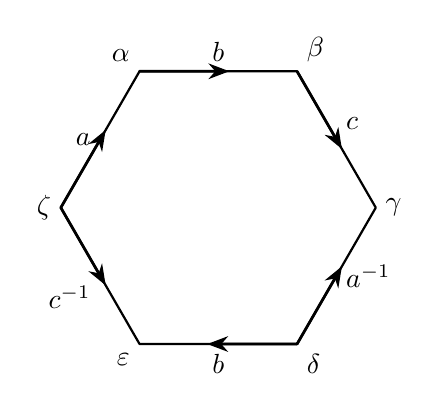
\begin{tikzpicture}[scale=2, line cap=round, line join=round]
    \coordinate (P0) at ({cos(120)},  {sin(120)});
    \coordinate (P1) at ({cos(60)},   {sin(60)});
    \coordinate (P2) at ({cos(0)},    {sin(0)});
    \coordinate (P3) at ({cos(-60)},  {sin(-60)});
    \coordinate (P4) at ({cos(-120)}, {sin(-120)});
    \coordinate (P5) at ({cos(180)},  {sin(180)});

    \node[above left]  at (P0) {$\alpha$};
    \node[above right] at (P1) {$\beta$};
    \node[right]       at (P2) {$\gamma$};
    \node[below right] at (P3) {$\delta$};
    \node[below left]  at (P4) {$\veps$};
    \node[left]        at (P5) {$\zeta$};
  
    \draw[thick] (P0)--(P1)--(P2)--(P3)--(P4)--(P5)--cycle;

    \tikzset{arr/.style={->, line width=1pt, >=Stealth}}

    \path (P5)--(P0) node[midway, left] {$a$};
    \draw[arr] (P5) -- ($(P5)!0.57!(P0)$);
    
    \path (P0)--(P1) node[midway, above] {$b$};
    \draw[arr] (P0) -- ($(P0)!0.57!(P1)$);

    \path (P1)--(P2) node[midway, above right] {$c$};
    \draw[arr] (P1) -- ($(P1)!0.57!(P2)$);

    \path (P2)--(P3) node[midway, right] {$a\inv$};
    \draw[arr] (P3) -- ($(P3)!0.57!(P2)$);

    \path (P3)--(P4) node[midway, below] {$b$};
    \draw[arr] (P3) -- ($(P3)!0.57!(P4)$);

    \path (P4)--(P5) node[midway, below left] {$c\inv$};
    \draw[arr] (P5) -- ($(P5)!0.57!(P4)$);
  \end{tikzpicture}
  \caption{A drawing of the polygon represented by the word $abca\inv bc\inv$}
\end{center}\end{figure}\vspace{-1em}

A word describes an orientable surface if and only if every symbol appears with both signs. \\
${}^{}$\hspace{1em}$a$ appears with both signs. $c$ appears with both signs. \\
${}^{}$\hspace{1em}However, $b$ only appears with one sign. \\
Therefore, this word describes a non-orientable surface. \vspace{0.5em}

$F = 1$ face, trivially. \\
The word has length $6=2\cd3\iff n = 3$. \\
$E = n = 3$ edges. \\
Calculating the vertices now,\\
${}^{}$\hspace{1em}Let's start with $a$ and $a\inv$. We note that $\alpha\liff\gamma$ and $\zeta\liff\delta$. \\
${}^{}$\hspace{1em}Next we'll consider $b$ and $b$. We note that $\alpha\liff\delta$ and $\beta\liff\veps$. \\
${}^{}$\hspace{1em}Finally, let's consider $c$ and $c\inv$, and note $\beta\liff\zeta$ and $\gamma\liff\veps$. \\
All together, we have
$$
  \alpha\liff\gamma\liff\veps\liff\beta\liff\zeta\liff\delta
$$
Therefore, the surface has 1 vertex. $V=1$ vertex. \\
Therefore, the surface has Euler characteristic, $\chi = V - E + F = 1 - 3 + 1 = -1$. \vspace{0.5em}

Therefore, a non-orientable surface with $\chi=-1 = 2-g \iff g=3$, is the connected sum of 3 projective planes, by the classification theorem.

\newpage
\sol (b) \vspace{0.5em}
\begin{figure}[H]\begin{center}
  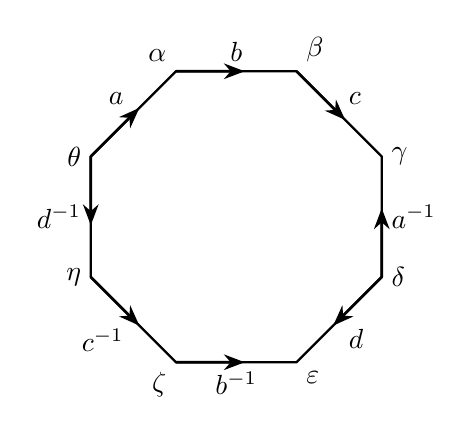
\begin{tikzpicture}[scale=2, line cap=round, line join=round]
    \coordinate (P0) at ({cos(112.5)},  {sin(112.5)});  
    \coordinate (P1) at ({cos(67.5)},   {sin(67.5)});   
    \coordinate (P2) at ({cos(22.5)},   {sin(22.5)});   
    \coordinate (P3) at ({cos(-22.5)},  {sin(-22.5)}); 
    \coordinate (P4) at ({cos(-67.5)},  {sin(-67.5)});  
    \coordinate (P5) at ({cos(-112.5)}, {sin(-112.5)}); 
    \coordinate (P6) at ({cos(-157.5)}, {sin(-157.5)}); 
    \coordinate (P7) at ({cos(-202.5)}, {sin(-202.5)});

    \node[above left]  at (P0) {$\alpha$};
    \node[above right] at (P1) {$\beta$};
    \node[right]       at (P2) {$\gamma$};
    \node[right] at (P3) {$\delta$};
    \node[below right]  at (P4) {$\veps$};
    \node[below left]        at (P5) {$\zeta$};
    \node[left]        at (P6) {$\eta$};
    \node[left]        at (P7) {$\theta$};
  
    \draw[thick] (P0)--(P1)--(P2)--(P3)--(P4)--(P5)--(P6)--(P7)--cycle;

    \tikzset{arr/.style={->, line width=1pt, >=Stealth}}

    \path (P7)--(P0) node[midway, above left] {$a$};
    \draw[arr] (P7) -- ($(P7)!0.57!(P0)$);
    
    \path (P0)--(P1) node[midway, above] {$b$};
    \draw[arr] (P0) -- ($(P0)!0.57!(P1)$);

    \path (P1)--(P2) node[midway, above right] {$c$};
    \draw[arr] (P1) -- ($(P1)!0.57!(P2)$);

    \path (P2)--(P3) node[midway, right] {$a\inv$};
    \draw[arr] (P3) -- ($(P3)!0.57!(P2)$);

    \path (P3)--(P4) node[midway, below right] {$d$};
    \draw[arr] (P3) -- ($(P3)!0.57!(P4)$);

    \path (P4)--(P5) node[midway, below] {$b\inv$};
    \draw[arr] (P5) -- ($(P5)!0.57!(P4)$);

    \path (P5)--(P6) node[midway, below left] {$c\inv$};
    \draw[arr] (P6) -- ($(P6)!0.57!(P5)$);

    \path (P6)--(P7) node[midway, left] {$d\inv$};
    \draw[arr] (P7) -- ($(P7)!0.57!(P6)$);
  \end{tikzpicture}
  \caption{A drawing of the polygon represented by the word $abca\inv db\inv c\inv d\inv$}
\end{center}\end{figure}\vspace{-1em}

A word describes an orientable surface if and only if every symbol appears with both signs. \\
${}^{}$\hspace{1em}$a$ appears with both signs. \\
${}^{}$\hspace{1em}$b$ appears with both signs. \\
${}^{}$\hspace{1em}$c$ appears with both signs. \\
${}^{}$\hspace{1em}$d$ appears with both signs. \\
Therefore, this word describes a orientable surface. \vspace{0.5em}

$F = 1$ face, trivially. \\
The word has length $8=2\cd4\iff n = 4$. \\
$E = n = 4$ edges. \\
Calculating the vertices now,\\
${}^{}$\hspace{1em}Let's start with $a$ and $a\inv$. We note that $\alpha\liff\gamma$ and $\theta\liff\delta$. \\
${}^{}$\hspace{1em}Next we'll consider $b$ and $b\inv$. We note that $\beta\liff\veps$ and $\alpha\liff\zeta$. \\
${}^{}$\hspace{1em}Next we'll consider $c$ and $c\inv$. We note that $\gamma\liff\zeta$ and $\beta\liff\eta$. \\
${}^{}$\hspace{1em}Finally, let's consider $d$ and $d\inv$, and note $\veps\liff\eta$ and $\delta\liff\theta$. \\
All together, we have
$$
  \alpha\liff\gamma\liff\zeta,\qquad\theta\liff\delta,\qquad\beta\liff\veps\liff\eta
$$
Therefore, the polygon has 3 vertices. \\
$V=3$ vertices. \\
Therefore, the polygon has Euler characteristic, $\chi = V - E + F = 3 - 4 + 1 = 0$. \vspace{0.5em}

Therefore, a orientable surface with $\chi=0 = 2-2g \iff g=1$, is the connected sum of 1 torus, by the classification theorem, ie, a torus.

\newpage
\qs{5 marks}{
  Consider the closed surface represented by the following word: 
  \[
    a\,b\,c\,a^{-1}\,d\,b\,c^{-1}\,d^{-1}.
  \]
  Use the word rules from  lectures to  identify the surface in the form stated in the classification theorem.
  }
\sol\vspace{0.5em}

Firstly, we'll note that $b$ appears with only one sign, hence the surface the word represents is non-orientable. \vspace{-1em}
\begin{align*}
  \intertext{We'll start transforming the word by applying rule 6, ``moving outside $xx$ pairs,'' to the two $b$'s.}
  a\,b\,c\,a\inv\,d\,b\,c\inv\,d\inv &\stackrel{r.6}{=} a\,b\,b\,d\inv\,a\,c\inv\,c\inv\,d\inv
  \intertext{We'll then apply rule 6 again to the two $d\inv$'s.}
  a\,b\,b\,d\inv\,a\,c\inv\,c\inv\,d\inv &\stackrel{r.6}{=} a\,b\,b\,d\inv\,d\inv\,c\,c\,a\inv
  \intertext{Next, we'll apply rule 2, ``cycling edges,'' to move the $a\inv$ to the front of the word.}
  a\,b\,b\,d\inv\,d\inv\,c\,c\,a\inv &\stackrel{r.2}{=} a\inv\,a\,b\,b\,d\inv\,d\inv\,c\,c
  \intertext{For the sake of sematics (not-shortcutting anything), we'll apply rule 1, ``relabelling edges,'' to swap around $a$ and $a\inv$.}
  a\inv\,a\,b\,b\,d\inv\,d\inv\,c\,c &\stackrel{r.1}{=} a\,a\inv\,b\,b\,d\inv\,d\inv\,c\,c
  \intertext{Now, we can apply rule 5, ``cancelling $xx\inv$ pairs'' to cancel out the $aa\inv$ at the front of the word.}
  a\,a\inv\,b\,b\,d\inv\,d\inv\,c\,c &\stackrel{r.5}{=} b\,b\,d\inv\,d\inv\,c\,c
  \intertext{Finally, we'll clean this up by applying rule 1 twice: to relabel $b$ as $a$; and to relabel $d\inv$ as $b$.}
  b\,b\,d\inv\,d\inv\,c\,c &\stackrel{r.1}{=} a\,a\,b\,b\,c\,c
\end{align*}
In accordance with the classification theorem, the word $abca^{-1}dbc^{-1}d^{-1}$, therefore, represents a surface which is non-orientable and the sum of 3 projective planes with Euler characteristic $-1$.

\newpage
\qs{8 marks}{
  Consider the sequence $S=(5,3,3,3,1,1)$.
  \begin{enumerate}[label=(\alph*), itemsep=0pt]
    \item Show that $S$ is graphical, and draw a graph with the degree sequence $S$.
    \item Prove that the graph with the degree sequence $S$ is unique up to graph isomorphism.
  \end{enumerate}
}
\sol (a) \vspace{0.5em}

To show $S$ is graphical, we'll use Theorem 25.76. First, we'll note that $S$ is monotone decreasing ($d_1=5\geq d_2=3\geq ... \geq d_p = d_6 = 1$), with $p=6\geq2$ and $\Delta = 5\geq1$. Therefore, we can apply the theorem; the first reduction:
\[
  (5,3,3,3,1,1) \xrightarrow{Thm. 25.76} (3-1, 3-1, 3-1, 1-1, 1-1) = (2,2,2,0,0)
\]
The sequence is monotone decreasing, with $p=5\geq2$ and $\Delta=2\geq1$. The second reduction:
\[
  (2,2,2,0,0) \xrightarrow{Thm. 25.76} (2-1, 2-1, 0, 0) = (1,1,0,0)
\]
The sequence is monotone decreasing, with $p=4\geq2$ and $\Delta=1\geq1$. The third reduction:
\[
  (1,1,0,0) \xrightarrow{Thm. 25.76} (1-1, 0, 0) = (0,0,0)
\]
Because the $\Delta$ for this sequence is $0<1$, the recurrsion ceases, but this reduced graph is trivially graphical because it represents the degree sequence of some graph (namely, three vertices with no edges). Therefore, $S$ is graphical.

\begin{figure}[H]\begin{center}
  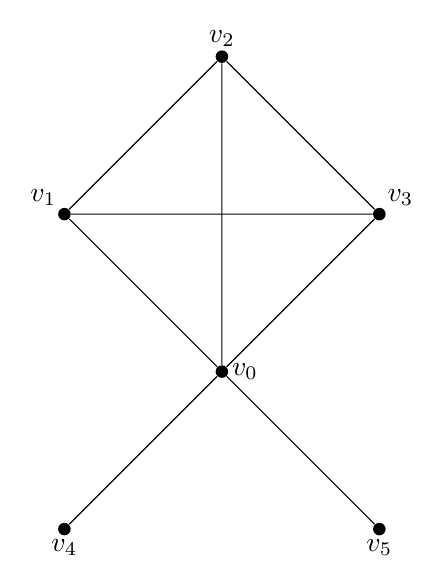
\begin{tikzpicture}[
    scale=2,
    v/.style={circle, fill=black, inner sep=1.6pt},
    every label/.style={inner sep=1pt}
  ]
    \node[v, label=right:$v_0$] (a) at (0,0) {};
    \node[v, label=above left:$v_1$] (b) at (-1,1) {};
    \node[v, label=above:$v_2$] (c) at (0,2) {};
    \node[v, label=above right:$v_3$] (d) at (1,1) {};
    \node[v, label=below:$v_4$] (e) at (-1,-1) {};
    \node[v, label=below:$v_5$] (f) at (1,-1) {};
    
    \draw (a)--(b) (a)--(c) (a)--(d) (a)--(e) (a)--(f);
    \draw (b)--(c) (d)--(c) (b)--(d);
  \end{tikzpicture}
  \caption{A drawing of a simple graph with degree sequence $S = (5,3,3,3,1,1)$.}
\end{center}\end{figure}\vspace{-1em}

\newpage
\sol (b) \vspace{0.5em}

\Claim\ The graph with degree sequence $S=(5,3,3,3,1,1)$ is unique up to graph isomorphism. \\
\Proof\ By construction.
\begin{list}{}{\setlength{\leftmargin}{0.6in}\setlength{\topsep}{0pt}}\item 
  The graph, $G$, with degree sequence $S$ is graphical.

  $\abs{S}=6$, hence $\abs{V(G)}=6$. \\
  $\Delta(S)=5 = \abs{V(G)}-1$, so the vertex with the greatest degree, call it $v_0$ has $d(v_0)=5$, and must be connected to all other vertices in the graph. \\
  Therefore, $\braces{\braces{v_0,v_1}, \braces{v_0,v_2}, \braces{v_0,v_3}, \braces{v_0,v_4}\braces{v_0,v_5}}= M \subseteq E(G)$.

  There are two vertices, call them $v_4$ and $v_5$ with $d(v_4)=d(v_5)=1$. \\
  The only choice for the other endpoint of these edges is $v_0$. \\
  These edges, namely $\braces{v_4,v_0}$ and $\braces{v_5,v_0}$, are already in the constructed set.

  The remaining three vertices, $v_1,\ v_2,\ v_3$ have $d(v_1)=d(v_2)=d(v_3)=3$. \\
  Each of these has one edge joining it to $v_0$, namely $\braces{v_1,v_0},\ \braces{v_2,v_0},\ \braces{v_3,v_0}$, all of which are already included in our constructed set. \\
  $v_1$ has 2 incident edges left to account for and only 2 choices: $v_2$ and $v_3$. \\
  $v_2$ has 2 incident edges left to account for and only 2 choices: $v_1$ and $v_3$. \\
  $v_3$ has 2 incident edges left to account for and only 2 choices: $v_1$ and $v_2$. \\
  Therefore, $\braces{\braces{v_1,v_2},\braces{v_1,v_3}}\cup\braces{\braces{v_2,v_1},\braces{v_2,v_3}}\cup\braces{\braces{v_3,v_1},\braces{v_3,v_1}}$ \\ $= \braces{\braces{v_1,v_2},\braces{v_1,v_3},\braces{v_2,v_3}} = T \subseteq E(G)$

  $M\cup T = \braces{\braces{v_0,v_1}, \braces{v_0,v_2}, \braces{v_0,v_3}, \braces{v_0,v_4}, \braces{v_0,v_5}, \braces{v_1,v_2}, \braces{v_1,v_3}, \braces{v_2,v_3}} \subseteq E(G)$

  By the Handshake Theorem, $\dps{\sum_{i=0}^{p-1}d(v_i) = d(v_0) + d(v_1) + d(v_2) + d(v_3) + d(v_4) + d(v_5)}$ \\ $= 5 + 3 + 3 + 3 + 1 + 1 = 16 = 2q\iff q=8$, therefore, $\abs{E(G)}=8$.

  $\abs{M \cup T} = 8$. 

  Therefore, $M\cup T = E(G)$.

  By our construction, this is the only graph with degree sequence $S$ (a consequence of the various forced decisions made throughout the process). \\
\end{list}
Therefore, the graph with degree sequence $S$ is unique up to graph isomorphism. $\QED$

\newpage
\qs{7 marks}{
  Suppose that $G$ is a graph on $4k+3$ vertices, where each vertex has degree at least $2k+1$, for some integer $k \geq 1$. 
  \begin{enumerate}[label=(\alph*), itemsep=0pt]
    \item  Can $G$ be $(2k+1)$-regular? Justify your answer. 
    \item  Prove that $G$ is connected. 
  \end{enumerate}
}
\sol (a) \vspace{0.3em}

Suppose $G$ were $(2k+1)$-regular. \\
Then it would be a graph with $4k+3$ vertices, where each vertex has degree $2k+1$. \vspace{0.3em}

Then, we could calculate this graph's degree total: 
\[
  (4k+3)(2k+1) = 8k^2+10k+3 = 2(4k^2+5k+1)+1 = 2z+1,\ z\in\bbz,
\]
which has odd parity. \vspace{0.3em}

We can also calculate this graphs degree total with the Handshake Theorem, namely:
\[
  \sum_{\forall v\in V(G)} d(v) = 2q,\ q\in\bbz,
\]
which has even parity.\vspace{0.3em}

Therefore, no $(2k+1)$-regular graph with $4k+3$ vertices exists, because of this clear contradiction.\\
Therefore, $G$ cannot be $(2k+1)$-regular. \\

\sol (b) \vspace{0.5em}

Suppose $G$ is a graph on $4k+3$ vertices such that each vertex has degree at least $2k+1$, for some integer $k\geq1$. \\
\Claim\ G is connected.
\proof\ By contradiction.
\begin{list}{}{\setlength{\leftmargin}{0.6in}\setlength{\topsep}{0pt}}\item 
  For the sake of contradiction, suppose that $G$ is disconected. \\
  Then $G$ can be decomposed into at least 2 connected subgraphs. 

  Let one of these components have $t$ vertices. \\
  Then each vertex in this component has degree at most $t-1$.

  Since, $\delta(G)\geq 2k+1,$ we know $t-1\geq 2k+1$,\ $t\geq 2k+2$.

  Now, since $G$ can be decomposed into \textit{at least} 2 components,
  \begin{equation*}
    \abs{V(G)}\geq 2(2k+2) = 4k+4 > 4k+3 = \abs{V(G)} \tag*{\CONTRA}
  \end{equation*}
  This is a clear contradiction because $V(G)$ must simultaneously be equal to $4k+3$ and greater than or equal to $4k+4$. Absurd. \\
  Therefore, $G$ is not disconected.  
\end{list}
Therefore, $G$ is connected. $\QED$


\end{document}
